\documentclass{standalone}
\usepackage{tikz}
\usepackage{ctex,siunitx}
\setCJKmainfont{Noto Serif CJK SC}
\usepackage{tkz-euclide}
\usepackage{amsmath}
\usetikzlibrary{patterns, calc}
\usetikzlibrary {decorations.pathmorphing, decorations.pathreplacing, decorations.shapes,}
\begin{document}
\small
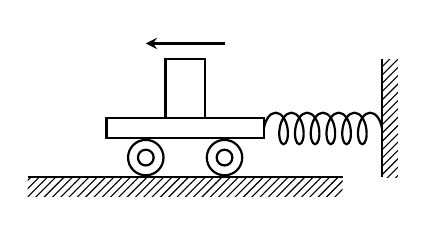
\begin{tikzpicture}[>=stealth, thick]
  \tikzstyle{spring}=[thick,decorate,decoration={aspect=0.5, segment length=2mm, amplitude=2mm,coil}]
  \useasboundingbox(-1,-0.75)rectangle(3.7,1.4);
  \draw [<-](0.5,1.2)--(1.5,1.2);
  \draw (0,0) rectangle (2,.25);
  \draw (.75,.25) rectangle (1.25,1);
  \fill [pattern = north east lines] (-1,-.75) rectangle (3,-.5);
  \fill [pattern = north east lines] (3.5,-.5) rectangle (3.7,1);
  \draw (3.5,-.5)--(3.5,1);
  \draw(-1,-.5)--(3,-.5);
  \draw (.5,-.25) circle (.225);
  \draw (1.5,-.25) circle (.225);
  \draw (.5,-.25) circle (.1);
  \draw (1.5,-.25) circle (.1);
  \draw [spring](2,.12)--(3.5,.12);
  \end{tikzpicture}
\end{document}